\documentclass[conference]{IEEEtran}
\usepackage[style=ieee, backend=biber]{biblatex}
\usepackage[T1]{fontenc}

\ifCLASSINFOpdf
	\usepackage[pdftex]{graphicx}
	\graphicspath{{img/}}
	\DeclareGraphicsExtensions{.pdf,.jpg,.png, .eps}
\else
	\usepackage[dvips]{graphicx}
 	\graphicspath{{img/}}
	\DeclareGraphicsExtensions{.pdf,.jpg,.png, .eps}
\fi


% *** MATH PACKAGES ***
%
%\usepackage{amsmath}
% A popular package from the American Mathematical Society that provides
% many useful and powerful commands for dealing with mathematics.
%
% Note that the amsmath package sets \interdisplaylinepenalty to 10000
% thus preventing page breaks from occurring within multiline equations. Use:
%\interdisplaylinepenalty=2500
% after loading amsmath to restore such page breaks as IEEEtran.cls normally
% does. amsmath.sty is already installed on most LaTeX systems. The latest
% version and documentation can be obtained at:
% http://www.ctan.org/pkg/amsmath





% *** SPECIALIZED LIST PACKAGES ***
%
%\usepackage{algorithmic}
% algorithmic.sty was written by Peter Williams and Rogerio Brito.
% This package provides an algorithmic environment fo describing algorithms.
% You can use the algorithmic environment in-text or within a figure
% environment to provide for a floating algorithm. Do NOT use the algorithm
% floating environment provided by algorithm.sty (by the same authors) or
% algorithm2e.sty (by Christophe Fiorio) as the IEEE does not use dedicated
% algorithm float types and packages that provide these will not provide
% correct IEEE style captions. The latest version and documentation of
% algorithmic.sty can be obtained at:
% http://www.ctan.org/pkg/algorithms
% Also of interest may be the (relatively newer and more customizable)
% algorithmicx.sty package by Szasz Janos:
% http://www.ctan.org/pkg/algorithmicx




% *** ALIGNMENT PACKAGES ***
%
%\usepackage{array}
% Frank Mittelbach's and David Carlisle's array.sty patches and improves
% the standard LaTeX2e array and tabular environments to provide better
% appearance and additional user controls. As the default LaTeX2e table
% generation code is lacking to the point of almost being broken with
% respect to the quality of the end results, all users are strongly
% advised to use an enhanced (at the very least that provided by array.sty)
% set of table tools. array.sty is already installed on most systems. The
% latest version and documentation can be obtained at:
% http://www.ctan.org/pkg/array


% IEEEtran contains the IEEEeqnarray family of commands that can be used to
% generate multiline equations as well as matrices, tables, etc., of high
% quality.




% *** SUBFIGURE PACKAGES ***
%\ifCLASSOPTIONcompsoc
%  \usepackage[caption=false,font=normalsize,labelfont=sf,textfont=sf]{subfig}
%\else
%  \usepackage[caption=false,font=footnotesize]{subfig}
%\fi
% subfig.sty, written by Steven Douglas Cochran, is the modern replacement
% for subfigure.sty, the latter of which is no longer maintained and is
% incompatible with some LaTeX packages including fixltx2e. However,
% subfig.sty requires and automatically loads Axel Sommerfeldt's caption.sty
% which will override IEEEtran.cls' handling of captions and this will result
% in non-IEEE style figure/table captions. To prevent this problem, be sure
% and invoke subfig.sty's "caption=false" package option (available since
% subfig.sty version 1.3, 2005/06/28) as this is will preserve IEEEtran.cls
% handling of captions.
% Note that the Computer Society format requires a larger sans serif font
% than the serif footnote size font used in traditional IEEE formatting
% and thus the need to invoke different subfig.sty package options depending
% on whether compsoc mode has been enabled.
%
% The latest version and documentation of subfig.sty can be obtained at:
% http://www.ctan.org/pkg/subfig




% *** FLOAT PACKAGES ***
%
%\usepackage{fixltx2e}
% fixltx2e, the successor to the earlier fix2col.sty, was written by
% Frank Mittelbach and David Carlisle. This package corrects a few problems
% in the LaTeX2e kernel, the most notable of which is that in current
% LaTeX2e releases, the ordering of single and double column floats is not
% guaranteed to be preserved. Thus, an unpatched LaTeX2e can allow a
% single column figure to be placed prior to an earlier double column
% figure.
% Be aware that LaTeX2e kernels dated 2015 and later have fixltx2e.sty's
% corrections already built into the system in which case a warning will
% be issued if an attempt is made to load fixltx2e.sty as it is no longer
% needed.
% The latest version and documentation can be found at:
% http://www.ctan.org/pkg/fixltx2e


%\usepackage{stfloats}
% stfloats.sty was written by Sigitas Tolusis. This package gives LaTeX2e
% the ability to do double column floats at the bottom of the page as well
% as the top. (e.g., "\begin{figure*}[!b]" is not normally possible in
% LaTeX2e). It also provides a command:
%\fnbelowfloat
% to enable the placement of footnotes below bottom floats (the standard
% LaTeX2e kernel puts them above bottom floats). This is an invasive package
% which rewrites many portions of the LaTeX2e float routines. It may not work
% with other packages that modify the LaTeX2e float routines. The latest
% version and documentation can be obtained at:
% http://www.ctan.org/pkg/stfloats
% Do not use the stfloats baselinefloat ability as the IEEE does not allow
% \baselineskip to stretch. Authors submitting work to the IEEE should note
% that the IEEE rarely uses double column equations and that authors should try
% to avoid such use. Do not be tempted to use the cuted.sty or midfloat.sty
% packages (also by Sigitas Tolusis) as the IEEE does not format its papers in
% such ways.
% Do not attempt to use stfloats with fixltx2e as they are incompatible.
% Instead, use Morten Hogholm'a dblfloatfix which combines the features
% of both fixltx2e and stfloats:
%
% \usepackage{dblfloatfix}
% The latest version can be found at:
% http://www.ctan.org/pkg/dblfloatfix




% *** PDF, URL AND HYPERLINK PACKAGES ***
%
\usepackage{url}
% url.sty was written by Donald Arseneau. It provides better support for
% handling and breaking URLs. url.sty is already installed on most LaTeX
% systems. The latest version and documentation can be obtained at:
% http://www.ctan.org/pkg/url
% Basically, \url{my_url_here}.




% *** Do not adjust lengths that control margins, column widths, etc. ***
% *** Do not use packages that alter fonts (such as pslatex).         ***
% There should be no need to do such things with IEEEtran.cls V1.6 and later.
% (Unless specifically asked to do so by the journal or conference you plan
% to submit to, of course. )


% correct bad hyphenation here
\hyphenation{op-tical net-works semi-conduc-tor}


\bibliography{paper.bib}


\begin{document}
\title{Mimicry in Online Conversations: An Exploratory Study of Linguistic Analysis Techniques}


% author names and affiliations
% use a multiple column layout for up to three different
% affiliations
\author{\IEEEauthorblockN{Tom Carrick, Awais Rashid, Paul J Taylor}
\IEEEauthorblockA{Security Lancaster / CREST\\
Lancaster University\\
Lancaster, United Kingdom\\
Email: \{t.carrick, a.rashid, p.j.taylor\} @lancaster.ac.uk}}

% conference papers do not typically use \thanks and this command
% is locked out in conference mode. If really needed, such as for
% the acknowledgment of grants, issue a \IEEEoverridecommandlockouts
% after \documentclass

% for over three affiliations, or if they all won't fit within the width
% of the page, use this alternative format:
% 
%\author{\IEEEauthorblockN{Michael Shell\IEEEauthorrefmark{1},
%Homer Simpson\IEEEauthorrefmark{2},
%James Kirk\IEEEauthorrefmark{3}, 
%Montgomery Scott\IEEEauthorrefmark{3} and
%Eldon Tyrell\IEEEauthorrefmark{4}}
%\IEEEauthorblockA{\IEEEauthorrefmark{1}School of Electrical and Computer Engineering\\
%Georgia Institute of Technology,
%Atlanta, Georgia 30332--0250\\ Email: see http://www.michaelshell.org/contact.html}
%\IEEEauthorblockA{\IEEEauthorrefmark{2}Twentieth Century Fox, Springfield, USA\\
%Email: homer@thesimpsons.com}
%\IEEEauthorblockA{\IEEEauthorrefmark{3}Starfleet Academy, San Francisco, California 96678-2391\\
%Telephone: (800) 555--1212, Fax: (888) 555--1212}
%\IEEEauthorblockA{\IEEEauthorrefmark{4}Tyrell Inc., 123 Replicant Street, Los Angeles, California 90210--4321}}




% use for special paper notices
%\IEEEspecialpapernotice{(Invited Paper)}




% make the title area
\maketitle

% As a general rule, do not put math, special symbols or citations
% in the abstract
\begin{abstract}
The Interactive Alignment Model is the prevailing theory of linguistic alignment works from a psychological standpoint.
In this study we investigate how several linguistic alignment techniques can be used to detect mimicry at the lexical, syntactic and semantic levels of the Interactive Alignment Model.

We show that [something].
\end{abstract}


\IEEEpeerreviewmaketitle


\section{Introduction}

Mimicry in online conversations is an important and active area of research. Humans tend to mimic each other in many areas, such as speech \cite{levelt1982surface, bock1986syntactic, bock1989closed, garrod1987saying}, physical actions \cite{bernieri1988coordinated} and written text \cite{danescu2011chameleons, scissors2008linguistic}.

Existing research has shown that people who mimic each other’s language have more successful outcomes in joint tasks \cite{maddux2008chameleons}. Hence, detection of mimicry can be a valuable indicator in understanding group dynamics in collaborative settings. It can also play a role in other application areas, e.g., for detection of insider threats \cite{taylor2013detecting}.

There are a number of measures designed to capture mimicry in text, and some efforts have been made to compare and trial these techniques. However, few of these techniques are grounded in what cognitive  science knows about how mimicry works within humans.

This paper addresses this limitation by contrasting how well existing linguistic analysis techniques work to detect mimicry in relation to the Interactive Alignment Model. Further, we also consider some existing techniques that have not previously been used to detect mimicry and discuss their viability. The novel contributions of this paper are as follows:
\begin{itemize}
	\item We compare existing mimicry detection techniques and how they map to the Interactive Alignment Model 
	\item  We evaluate techniques that have not been used for mimicry detection before and discuss their feasibility in this regard.
	\item On the basis of our analysis, we posit that hybrid techniques, composing multiple measures, may offer a more holistic approach for mimicry detection.
\end{itemize}

Existing work has compared several methods, e.g., \cite{xu2015evaluation}, including some discussed in this paper. However, such works do not aim to contrast the effectiveness of the measures with regards to cognitive models such as the Interactive Alignment Model. To our knowledge, our work is the first to undertake such a comparison.

The rest of this paper is structured as follows. In Section II, we briefly introduce the Interactive Alignment Model - the psychological model of mimicry against which we test our techniques. Section III provides a brief introduction to each measure tested in the paper, and defines the layer of the IAM (if any) in which the measure resides. Section IV describes the data set used in our analysis. Section V presents the results of our analysis and highlights the importance of composing multiple measures. Finally, Section VI concludes the paper and identifies directions for future work.


\section{The Interactive Alignment Model}
The Interactive Alignment Model (IAM) \cite{pickering2004toward} is an attempt to model alignment in conversations. It consists of six layers, which with the exception of the top layer, the situation model, are all representations of some aspect of speech.

\begin{enumerate}
	\item The situation model --- a representation of the situation being discussed
	\item The semantic representation --- the meaning of the utterance
	\item The syntactic representation --- the sentence structure
	\item The lexical representation --- the choice of words used
	\item The phonological representation --- the abstract representation of word sounds
	\item The phonetic representation --- the sounds of an utterance
\end{enumerate}

The phonological and phonetic representations are not discussed in this paper as they relate purely to the sound of speech, representations that do not exist in the written text of online conversations.

Further, the situation model is not included as there are currently no measures that can be used for finding alignment at the situational level.

The theory states that alignment is automatic, that conversation partners will align their speech  towards each other at every level of the model. In addition, alignment "percolates" between layers such that increased alignment in one layer will lead to increased alignment in other layers.

\begin{figure*}
	\caption{The interactive alignment model}
	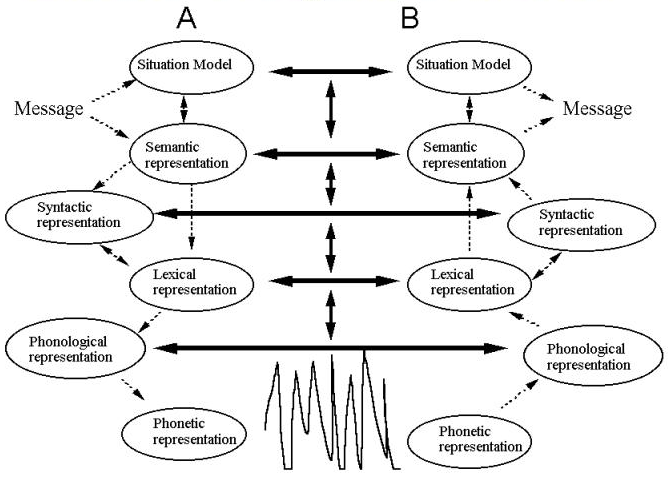
\includegraphics[width=\textwidth]{iam}
\end{figure*}


\section{Analysis Techniques}

There are many techniques that work at the lexical level, many of which can be re-purposed to be used at the syntactic level by replacing the words with phrase or dependency tree notation. One technique was used to represent each IAM layer, and one technique that works outside of the IAM.

The criteria for choosing techniques were:

\begin{itemize}
	\item Newer techniques were preferred over older ones.
	\item Availability of a source implementation or simplicity of implementation
\end{itemize}


\subsection{Local Linguistic Alignment}
Local Linguistic Alignment (LLA) is a simple,  dual purpose method that can work at both the lexical and syntactic layers \cite{wang2014linguistic, xu2015evaluation}.

Lexical Indiscriminate Local Linguistic Alignment (LILLA) works at the lexical layer. It gives the probability that a word from the prime document will appear at a particular position in the target  document. It is defined as:

\[LILLA(target, prime) = \frac{p(target|prime)}{p(target)}\]

Syntactic Indiscriminate Local Linguistic Alignemnt (SILLA) works at the syntactic layer. It works in exactly the same way as LILLA, but instead of comparing words, each sentence is annotated with a phrase structure tree, and LLA is run on these instead. As such, it measures the probability of a phrase structure subtree in the prime document appearing occurring at a given position in the target document.

\subsection{Word Vectors}
Word2vec \cite{mikolov2013efficient, mikolov2013distributed} is a machine learning technique that, given a word, tries to predict the two adjacent words. Each word is then mapped to vector space and can be directly compared. The closer the two word vectors to each other, the more semantically related they are.

While word vectors have not been used to measure mimicry before, we posit that it may give good results for finding mimicry as it gets good results in the related field of sentiment analysis and is used to find semantic similarity of texts.

\subsection{Language Style Matching}
Language Style Matching (LSM) \cite{ireland2010language, ireland2011language} is a measure that counts the usage of function words by an interlocutor. For each class of function word (e.g., determiners, pronouns, adpositions), the number of words is  calculated as a percentage of the total document, which is the score for each class. Scores are calculated between the dyad using a weighted difference, shown below, and these scores averaged to produce a single LSM score for that dyad.

\[ LSM_{class} = 1 - [(|class_1 - class_2|)] / (class_1 + class_2 + .0001) \]


\section{Method}
The dataset consists of 103 dyadic conversations taken from Twitter. Tweets were found via Twitter's  search API, using English language and being a reply as criteria. We then work up the chain of tweets  until we hit the end, or a third interlocutor is found, at which point the conversation is cut off and  kept, as long as there are no fewer than 10 tweets in the conversation. 200 tweets were found using  this method. Of these, 62 were removed as they were not true conversations (either monologues or  collaborative fiction writing/roleplay). 18 conversations were removed as they had significant amounts  of non-English text. 17 conversations involved bots and were also removed.

The data was processed as follows:
\begin{itemize}
	\item Screen names at the start of the message were removed. These are just the names of the 
		  interlocutors and only add noise.
	\item All URLs were replaced with the string '[URL]'.
	\item HTML entities such as \&amp; were converted to plain text (\&).
	\item Any adjacent messages by the same author were merged together such that each message always
	      alternates between the two interlocutors.
\end{itemize}

The dataset is small, which is both an advantage as it is possible to classify the data manually and a disadvantage in that the sample size is smaller. We did not actively seek out mimicry by targeting our search as it was important to have conversations that would test negatively for mimicry as well as positively.

The data was classified by three researchers with backgrounds in mimicry independent of the authors of  this paper. Each  conversation was classified for lexical, syntactic and semantic mimicry on a three point scale  where 0 represents no mimicry, 1 represents low levels of mimicry at that layer, and 2 represents high  levels of mimicry. Classifications from each author were averaged together to give each conversation three scores between 0 and 2.

Each measure was then run against the data such that each message from author A is compared with each  message from author B that occurred before the original message.

\footnote{[I could probably make my github repo public and put a link to the code here?]}


\section{Results}

In general, the human classifiers agreed with each other, but the agreement is fairly weak. They most strongly agreed on syntactic mimicry, \(r > 0.28, < 0.36, p < 0.004\). Additionally there seemed to be more agreement on lexical mimicry than semantic, but p values are too high to make a definitive judgment.

The mean scores from human classifiers also show positive but weak correlation with the scores from their respective techniques. Additionally means of all human classifier scores were used as a comparison with LSM. These correlations can be seen in Table \ref{scores_techniques}.

\begin{table}[!t]
\caption{Correlations of Classifier Scores and Techniques}
\label{scores_techniques}
\centering
\renewcommand{\arraystretch}{1.2}
\begin{tabular}{l c c}
Layer, Technique & r & p \\
\hline
Lexical, LILLA & 0.27 & 0.005 \\
Syntactic, SILLA & 0.19 & 0.057 \\
Semantic, Word2vec & 0.11 & 0.231 \\
N/A (mean scores), LSM & 0.16 & 0.111 \\
\end{tabular}
\end{table}

To observe the IAM's prediction that increased levels of mimicry on one layer results in a higher probability of mimicry in other adjacent layers, we looked at the correlations between the results of our techniques, in Table \ref{techniques}, and also between the results of the human classifiers, in Table \ref{classifications}.

\begin{table}[!t]
\caption{Correlations of Techniques}
\label{techniques}
\centering
\renewcommand{\arraystretch}{1.2}
\begin{tabular}{l c c}
Technique & r & p \\
\hline
LILLA, SILLA & 0.26 & 0.007 \\
LILLA, Word2vec & -0.31 & 0.002 \\
SILLA, Word2vec & -0.81 & < 0.001
\end{tabular}
\end{table}

\begin{table}[!t]
\caption{Correlations of Human Classifications}
\label{classifications}
\centering
\renewcommand{\arraystretch}{1.2}
\begin{tabular}{l c c}
Layer & r & p \\
\hline
Lexical, Syntactic & 0.57 & < 0.001 \\
Lexical, Semantic & 0.33 & < 0.001 \\
Syntactic, Semantic & 0.28 & 0.005
\end{tabular}
\end{table}



% An example of a floating figure using the graphicx package.
% Note that \label must occur AFTER (or within) \caption.
% For figures, \caption should occur after the \includegraphics.
% Note that IEEEtran v1.7 and later has special internal code that
% is designed to preserve the operation of \label within \caption
% even when the captionsoff option is in effect. However, because
% of issues like this, it may be the safest practice to put all your
% \label just after \caption rather than within \caption{}.
%
% Reminder: the "draftcls" or "draftclsnofoot", not "draft", class
% option should be used if it is desired that the figures are to be
% displayed while in draft mode.
%
%\begin{figure}[!t]
%\centering
%\includegraphics[width=2.5in]{myfigure}
% where an .eps filename suffix will be assumed under latex, 
% and a .pdf suffix will be assumed for pdflatex; or what has been declared
% via \DeclareGraphicsExtensions.
%\caption{Simulation results for the network.}
%\label{fig_sim}
%\end{figure}

% Note that the IEEE typically puts floats only at the top, even when this
% results in a large percentage of a column being occupied by floats.


% An example of a double column floating figure using two subfigures.
% (The subfig.sty package must be loaded for this to work.)
% The subfigure \label commands are set within each subfloat command,
% and the \label for the overall figure must come after \caption.
% \hfil is used as a separator to get equal spacing.
% Watch out that the combined width of all the subfigures on a 
% line do not exceed the text width or a line break will occur.
%
%\begin{figure*}[!t]
%\centering
%\subfloat[Case I]{\includegraphics[width=2.5in]{box}%
%\label{fig_first_case}}
%\hfil
%\subfloat[Case II]{\includegraphics[width=2.5in]{box}%
%\label{fig_second_case}}
%\caption{Simulation results for the network.}
%\label{fig_sim}
%\end{figure*}
%
% Note that often IEEE papers with subfigures do not employ subfigure
% captions (using the optional argument to \subfloat[]), but instead will
% reference/describe all of them (a), (b), etc., within the main caption.
% Be aware that for subfig.sty to generate the (a), (b), etc., subfigure
% labels, the optional argument to \subfloat must be present. If a
% subcaption is not desired, just leave its contents blank,
% e.g., \subfloat[].



\section{Discussion}
Discussion


\section{Conclusion and Future Work}
The conclusion goes here.
Zelig \cite{jones2014finding}


% use section* for acknowledgment
\section*{Acknowledgment}
This research is funded by the Engineering and Social Sciences (ESRC) Centre for Behavioural and Social Science Approaches to Security (CREST).


% trigger a \newpage just before the given reference
% number - used to balance the columns on the last page
% adjust value as needed - may need to be readjusted if
% the document is modified later
%\IEEEtriggeratref{8}
% The "triggered" command can be changed if desired:
%\IEEEtriggercmd{\enlargethispage{-5in}}

\printbibliography

\end{document}
